\section{ProtoDUNE-ND-Tracker: MINERvA components}
\label{sec:MINERvA}

This section discusses the ProtoDUNE-ND-Tracker components to be repurposed from the existing MINERvA detector, and forms the core of this proposal. The MINERvA experiment~\cite{minerva-nim}, which now controls and maintains the MINOS near detector, is located in the MINOS ND hall in which ProtoDUNE-ND will be installed, and is due to complete its data-taking in spring--summer 2019.

\subsection{Repurposing the MINERvA detector}
\label{sec:minerva}
The MINERvA detector is shown in Figure~\ref{fig:minerva_detector}. For the purpose of the discussion in this section, we will assume that the steel shield, scintillator veto plane, helium vessel, and nuclear targets region will be removed, and this setup will be referred to as the ``ProtoDUNE-ND-Tracker''.

\begin{figure}[htb]
  \centering
  \subfloat[Front view] {\label{fig:minerva_detector_front}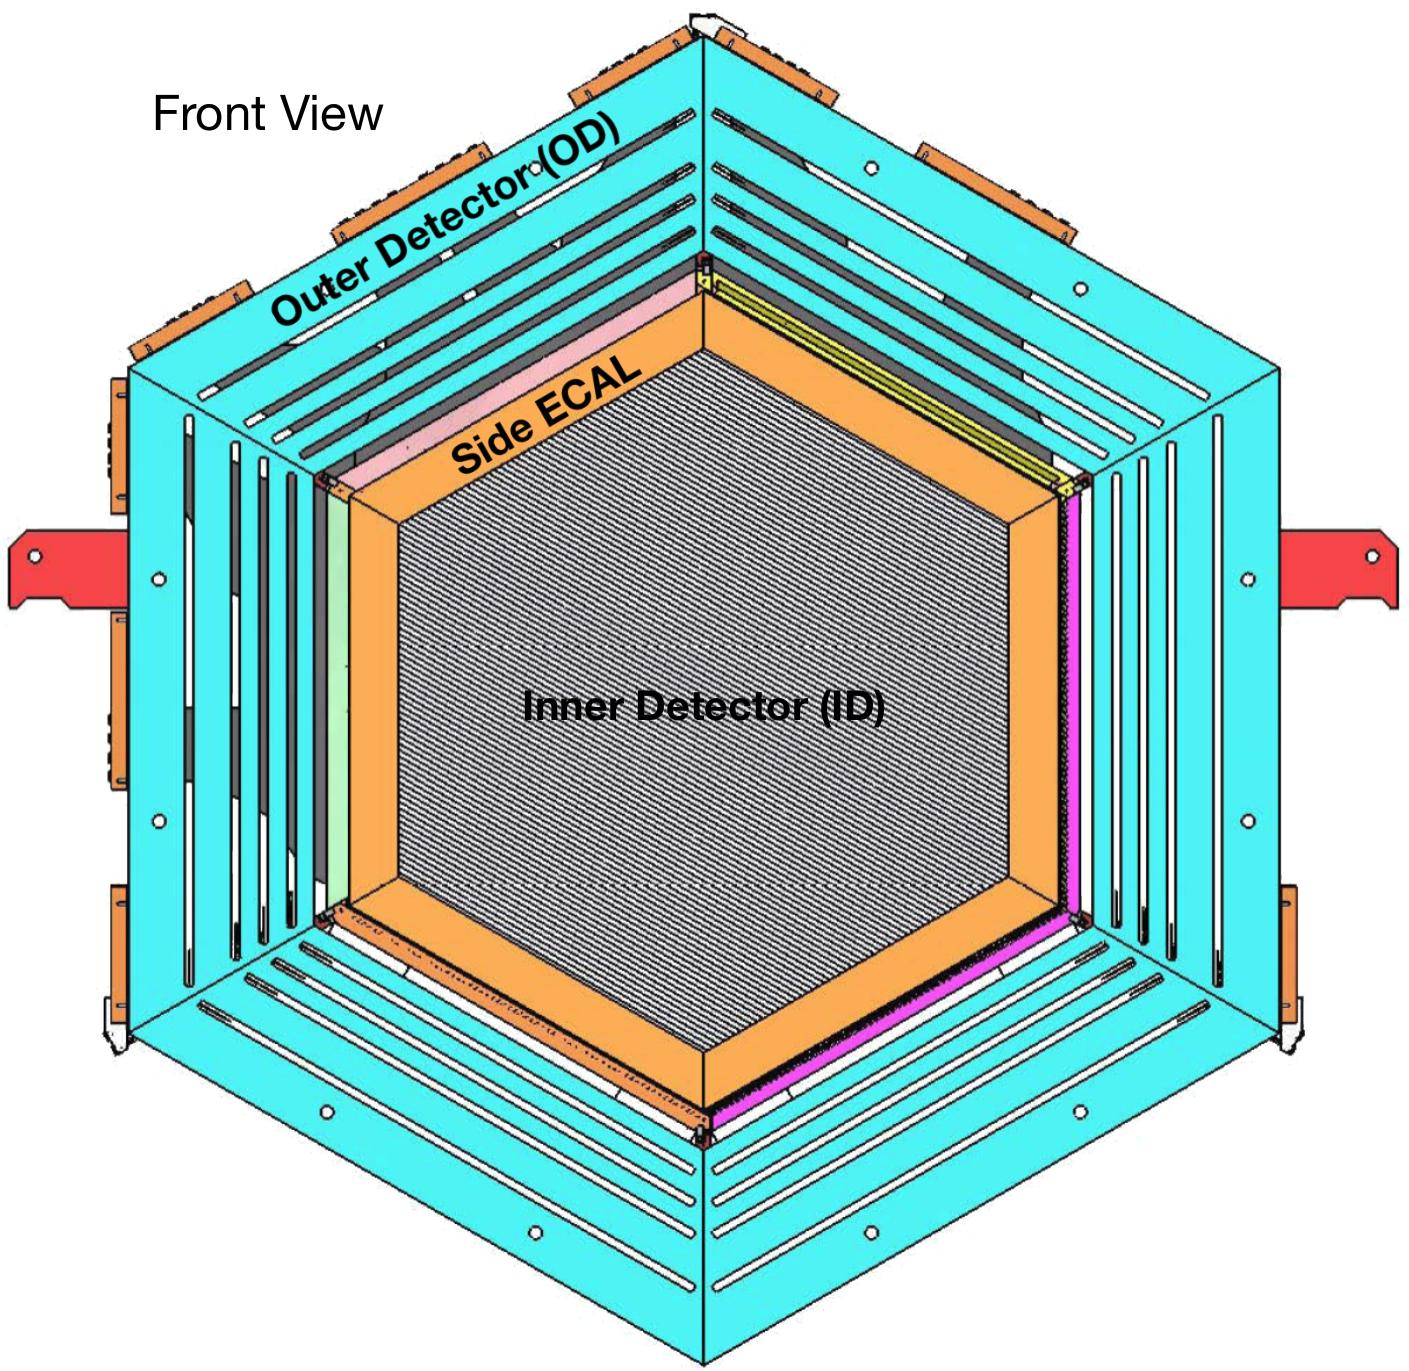
\includegraphics[width=0.35\textwidth]{plots/minerva_module_transverse}}
  \subfloat[Side view]  {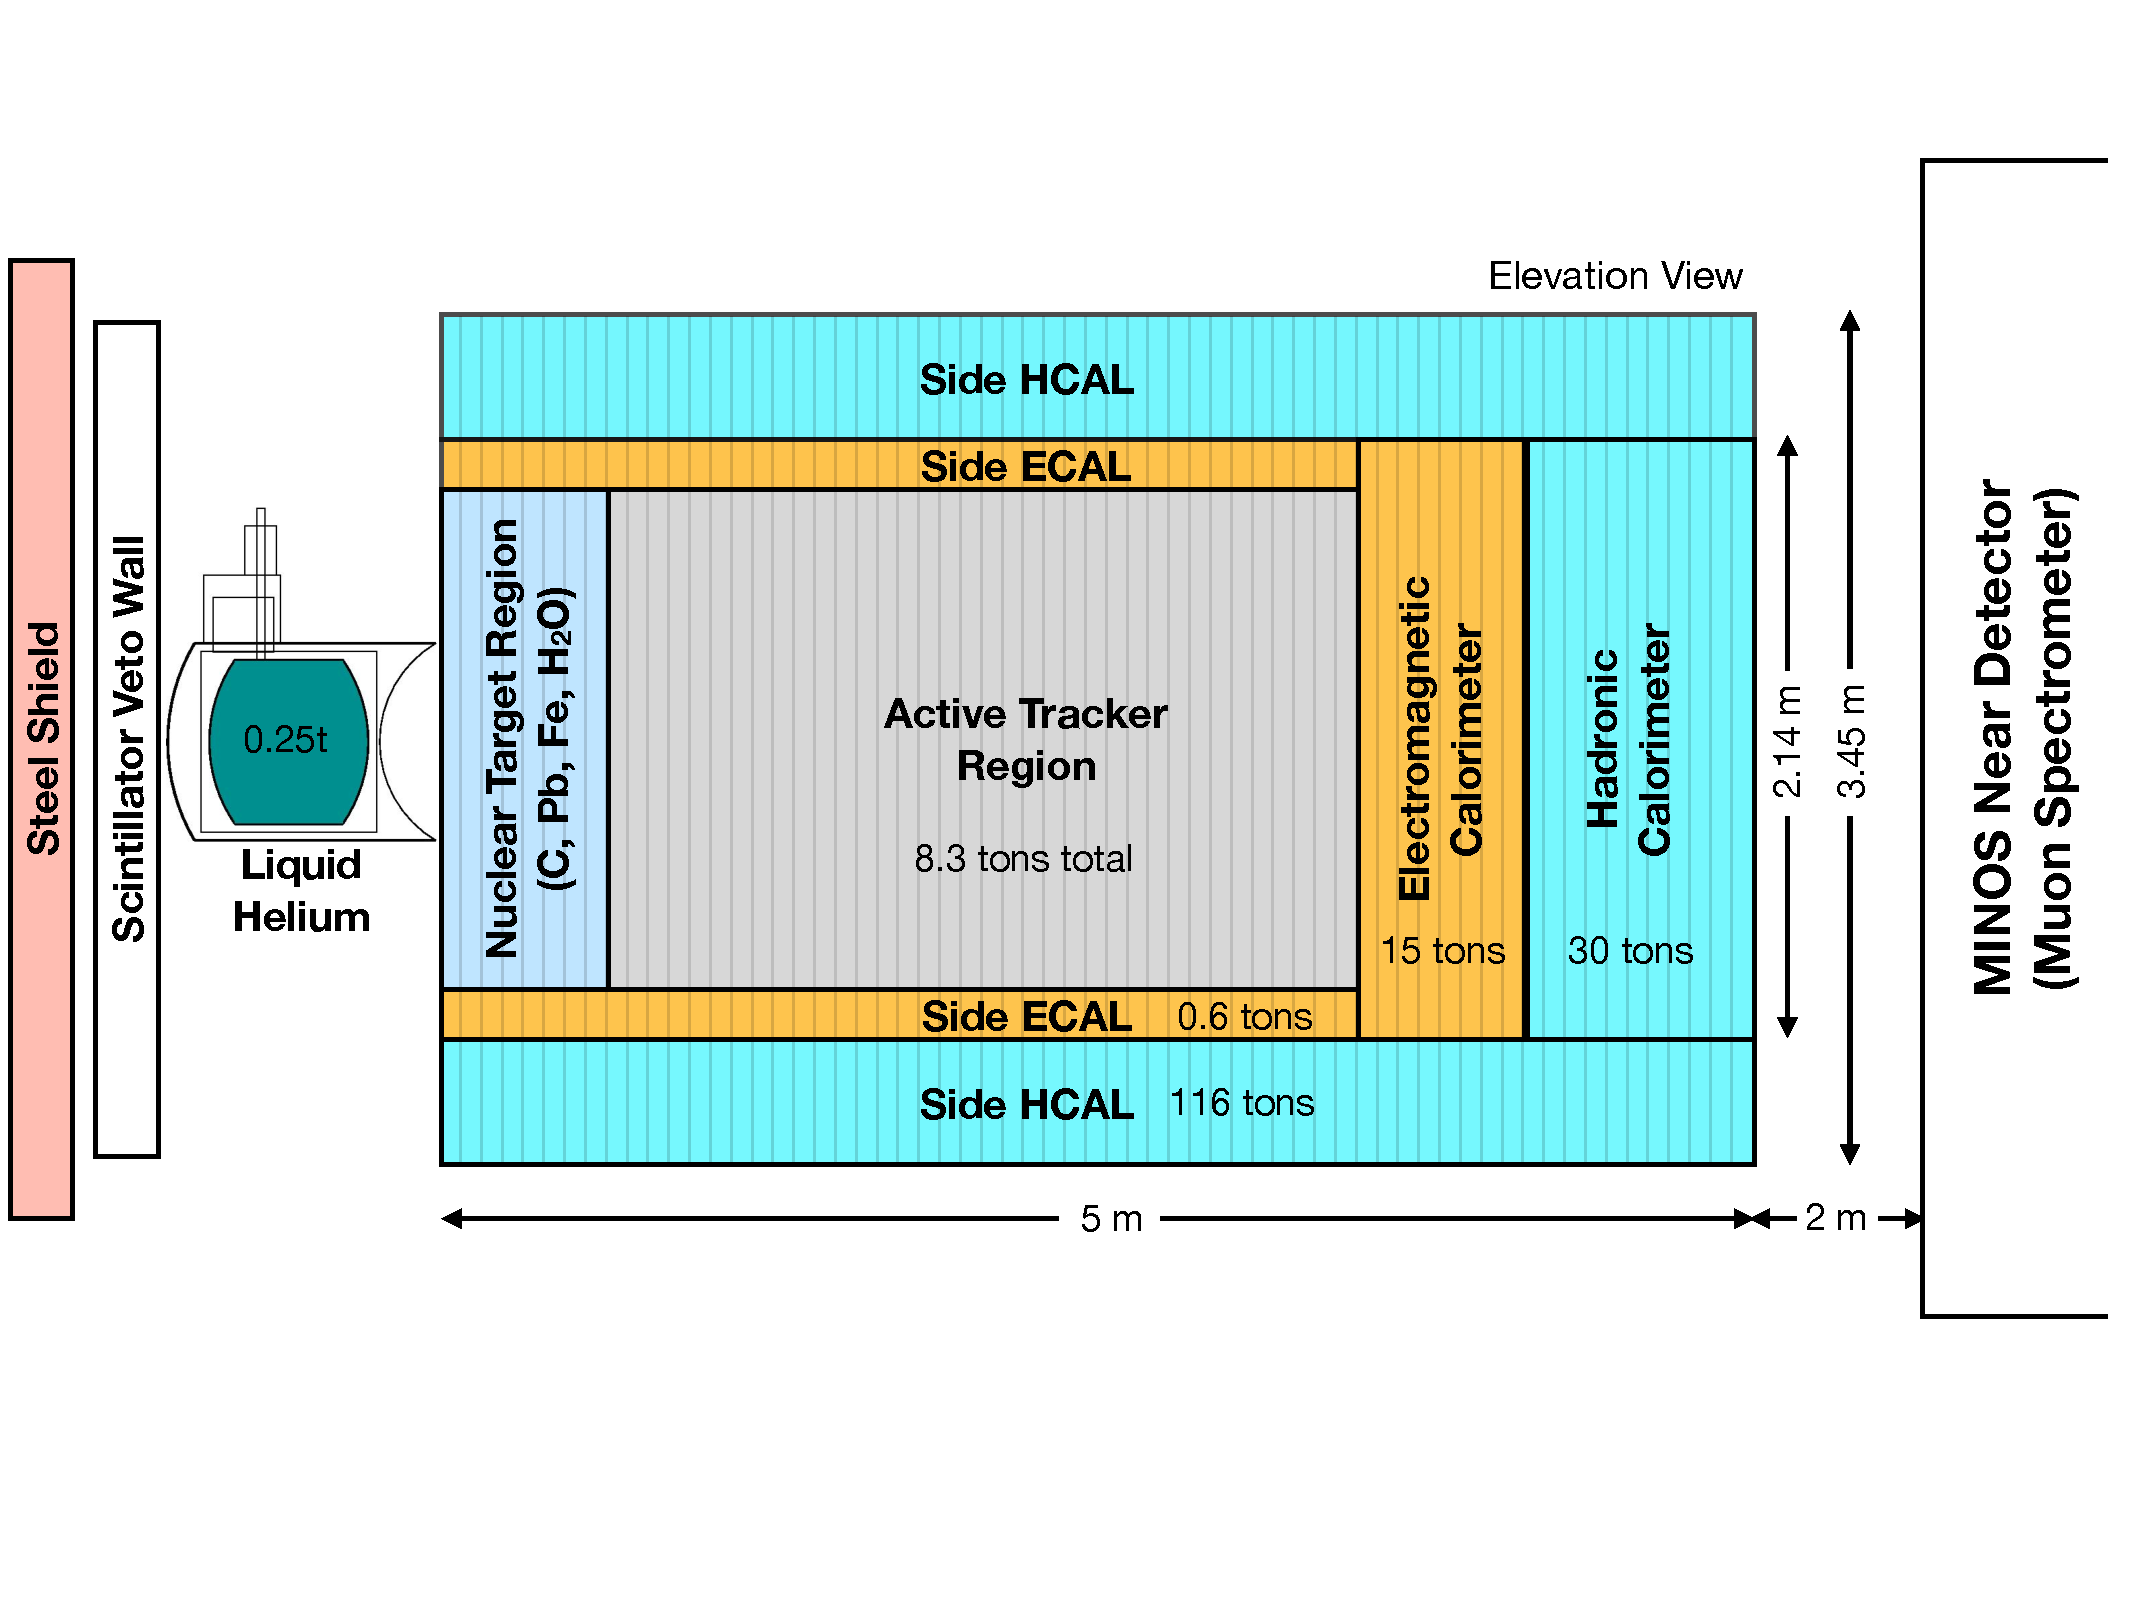
\includegraphics[width=0.60\textwidth]{plots/MINERvA_schematic.pdf}}
  \caption{Schematic of the MINERvA experiment. Reproduced from Figure 1 of Ref.~\cite{minerva-nim}.}
  \label{fig:minerva_detector}
\end{figure}

%Side is integral, and not separatable from central tracker.

The remaining central tracking region, and both the electromagnetic (EM) and hadronic calorimeters are divided into modules which consist mostly of hexagonal scintillator planes, each made of 127 triangular scintillator bars, arranged in three different orientations (60$^\circ$ rotations between each plane). There are 62 modules in the fully-active tracker region, each composed of two scintillator layers. A 15 cm border of 0.2 cm thick lead on the downstream end of each module provides EM calorimetry for particles exiting the side of the tracking region.

The downstream EM calorimeter is composed of 10 modules, each with two scintillator planes and a 0.2 cm thick lead plate on the downstream end. There are 20 modules in the downstream hadronic calorimeter, each with a single scintillator plane and a 2.54 cm thick hexagonal steel plane. The outer detector consists of a steel frame supporting structure with embedded scintillator planes, as can be seen in Figure~\ref{fig:minerva_detector_front}, which turns the support structure into a hadronic calorimeter. The combination of the downstream and side EM and hadronic calorimeters allows for containment of most particles which escape from the central tracking region, and allows for particle identification and momentum measurements.

\begin{figure}[htb]
  \centering
  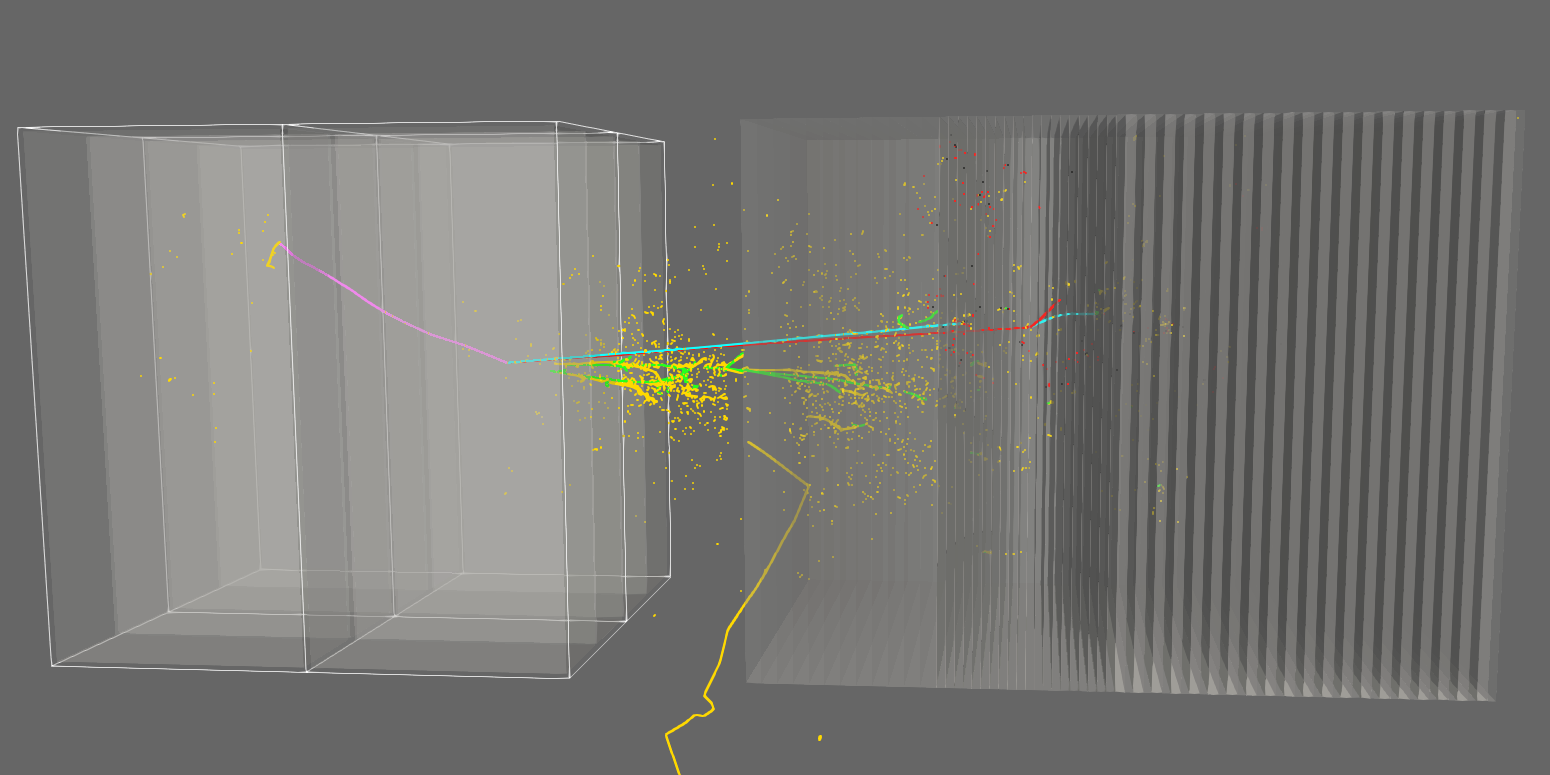
\includegraphics[width=0.8\textwidth]{{plots/Event_Displays_2x2_MINERvA/MINERvA_full_e70_rectangle_crop}.png}
  \caption{Example simulated event for a 7.0 GeV $\nu_{\mu}$--argon charged-current interaction, in which particles not contained in the ArgonCube 2x2 enter the ProtoDUNE-ND-Tracker downstream. Energy deposits are color-coded according to the particle type: $\pi^{\pm}$ --- blue; $\mu^{\pm}$ --- purple; $e^{+}$ --- green; $e^{-}$ --- yellow; proton --- red; recoiling nuclei --- black. The event vertex was randomly placed inside the active volume of the 2x2 Demonstrator module.}
  \label{fig:2x2+MINERvA_event}
\end{figure}

For the studies shown in this document, a simulation was performed approximating the downstream MINERvA central tracking region with a box of scintillator, and the ArgonCube 2x2 Demonstrator module upstream of the shortened MINERvA detector.
Neutrino interactions are generated in the ArgonCube active volume, and propagated through an approximation of the ArgonCube 2x2 demonstrator and partial MINERvA detector with a Geant4-based program\footnote{\url{https://github.com/dadwyer/argon_box}}.  
The MINERvA detector is approximated by a rectangular box, \SI[product-units=repeat]{1.4x1.4}{\metre\squared} in the dimensions transverse to the beam.  
The simulation includes the most downstream 12 modules (24 planes) of the tracker region, as well as the full downstream ECAL and HCAL regions.  
The rectangular box represents the central part of the MINERvA inner detector, and is large enough to cover the entire ArgonCube active volume. An example event is shown in Figure~\ref{fig:2x2+MINERvA_event}, and can be compared with ArgonCube 2x2-only events in Fig.~\ref{fig:leaky_event}, and in Ref.~\cite{2x2@FNAL} Fig. 7. Note that the ProtoDUNE-ND-Tracker simulation only includes the ArgonCube cryostat and repurposed MINERvA detector components, no material was included outside these (so escaping particles simply leave without ever re-interacting).

In the following, we discuss potential detector physics studies, or improvements to detector physics studies presented in Ref.~\cite{2x2@FNAL}, where we include ProtoDUNE-ND-Tracker downstream of the ArgonCube 2x2 module.

\subsection{Track matching}
All DUNE ND designs considered in Ref.~\cite{dune_ndcsg} include some fast scintillator component, downstream of the LAr ArgonCube component, and downstream of the HPgTPC, to tag escaping particles, photons, and possibly neutrons. There is a significant reconstruction challenge in matching the escaping tracks from the LAr component, with the signals in the scintillator, given the slow charge readout in the LAr TPC, and the high multiplicity DUNE-ND environment.

\begin{figure}[htb]
  \centering
  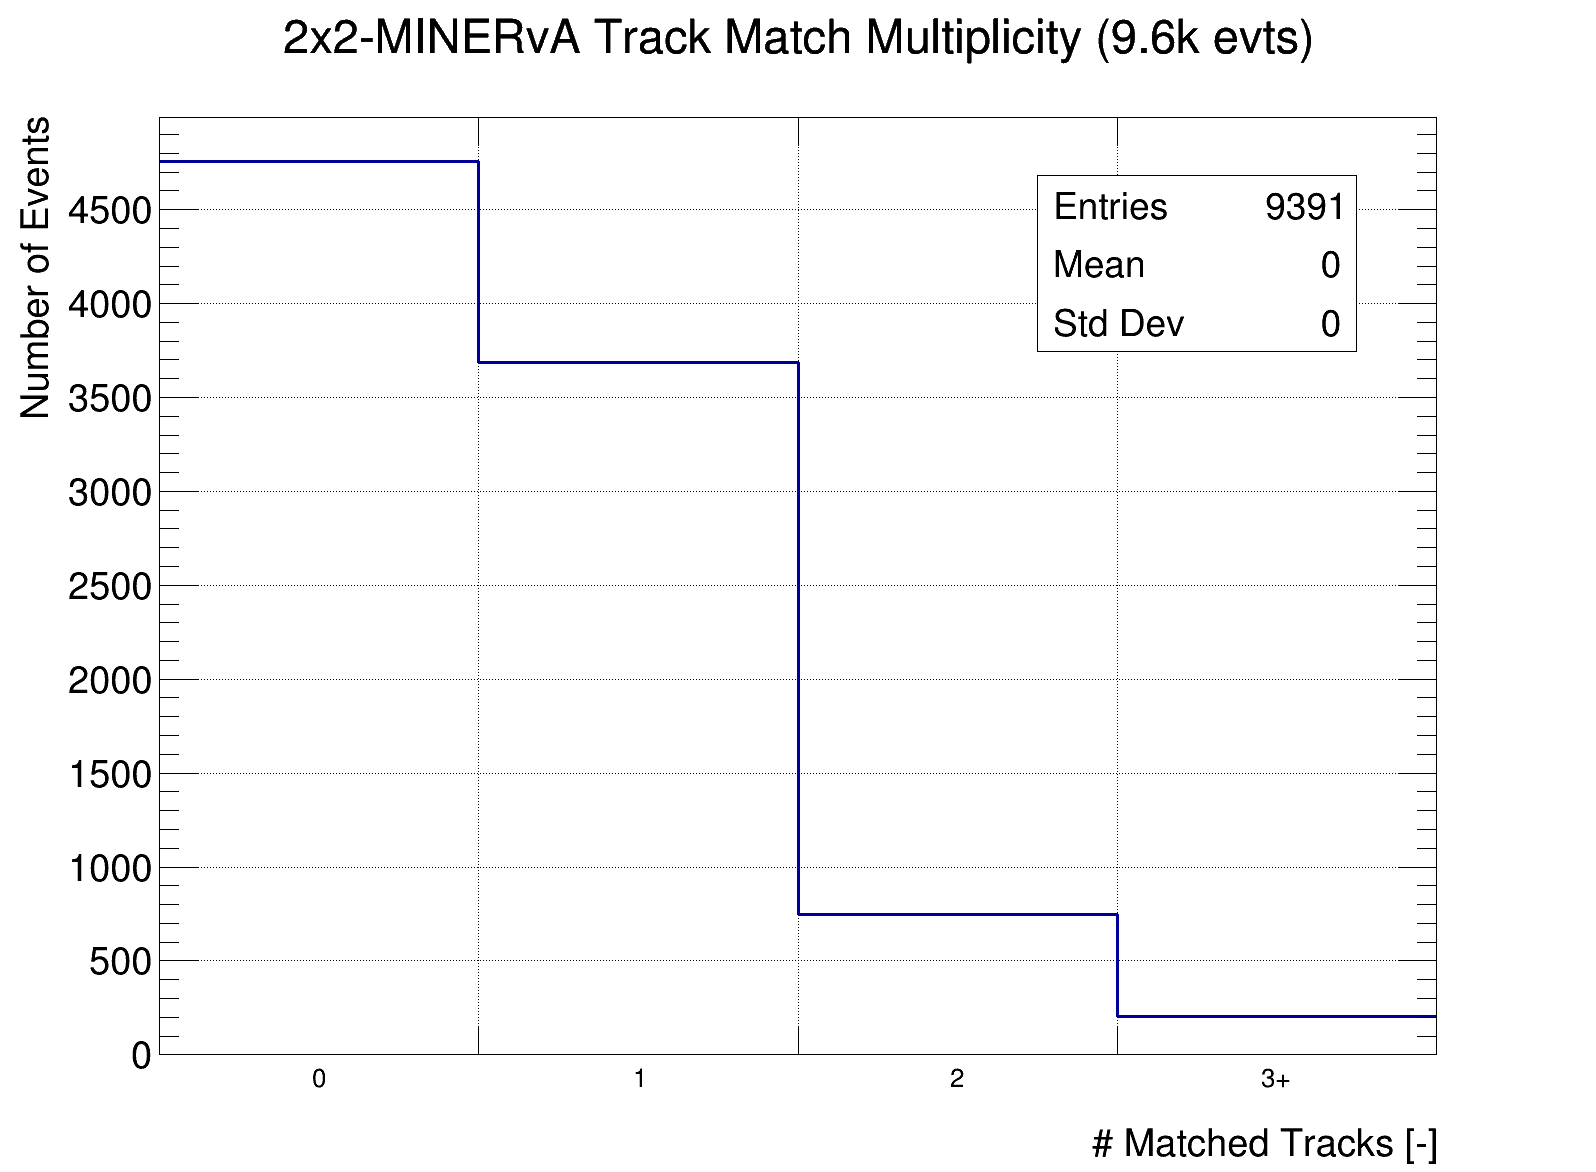
\includegraphics[width=0.6\textwidth]{plots/2x2_minerva_plots/track_mathch_multiplicity.png}
  \caption{Simulated number of true tracks produced by simulated GENIE interactions in the ArgonCube 2x2 active volume, which deposit energy in both the 2x2 module, and the ProtoDUNE-ND-Tracker positioned downstream of the 2x2.}
  \label{fig:track_multiplicity_min}
\end{figure}
Many tracks produced in the LAr volume are not contained by the ArgonCube 2x2 module, and the majority will escape downstream. In Figure~\ref{fig:hadronic_containment}, the multiplicity of tracks which deposit charge in both the ArgonCube 2x2 module and the ProtoDUNE-ND-Tracker, included in the simulation described above, are shown. Full DUNE-ND events are likely to have an even higher LAr to scintillator track multiplicity due to the pile-up in the much larger 35 t ArgonCube LAr detector. But it is clear from Figure~\ref{fig:track_multiplicity_min} that including the ProtoDUNE-ND-Tracker in ProtoDUNE-ND would provide useful data with which to start tackling this reconstruction problem.

\begin{figure}[htb]
  \centering
  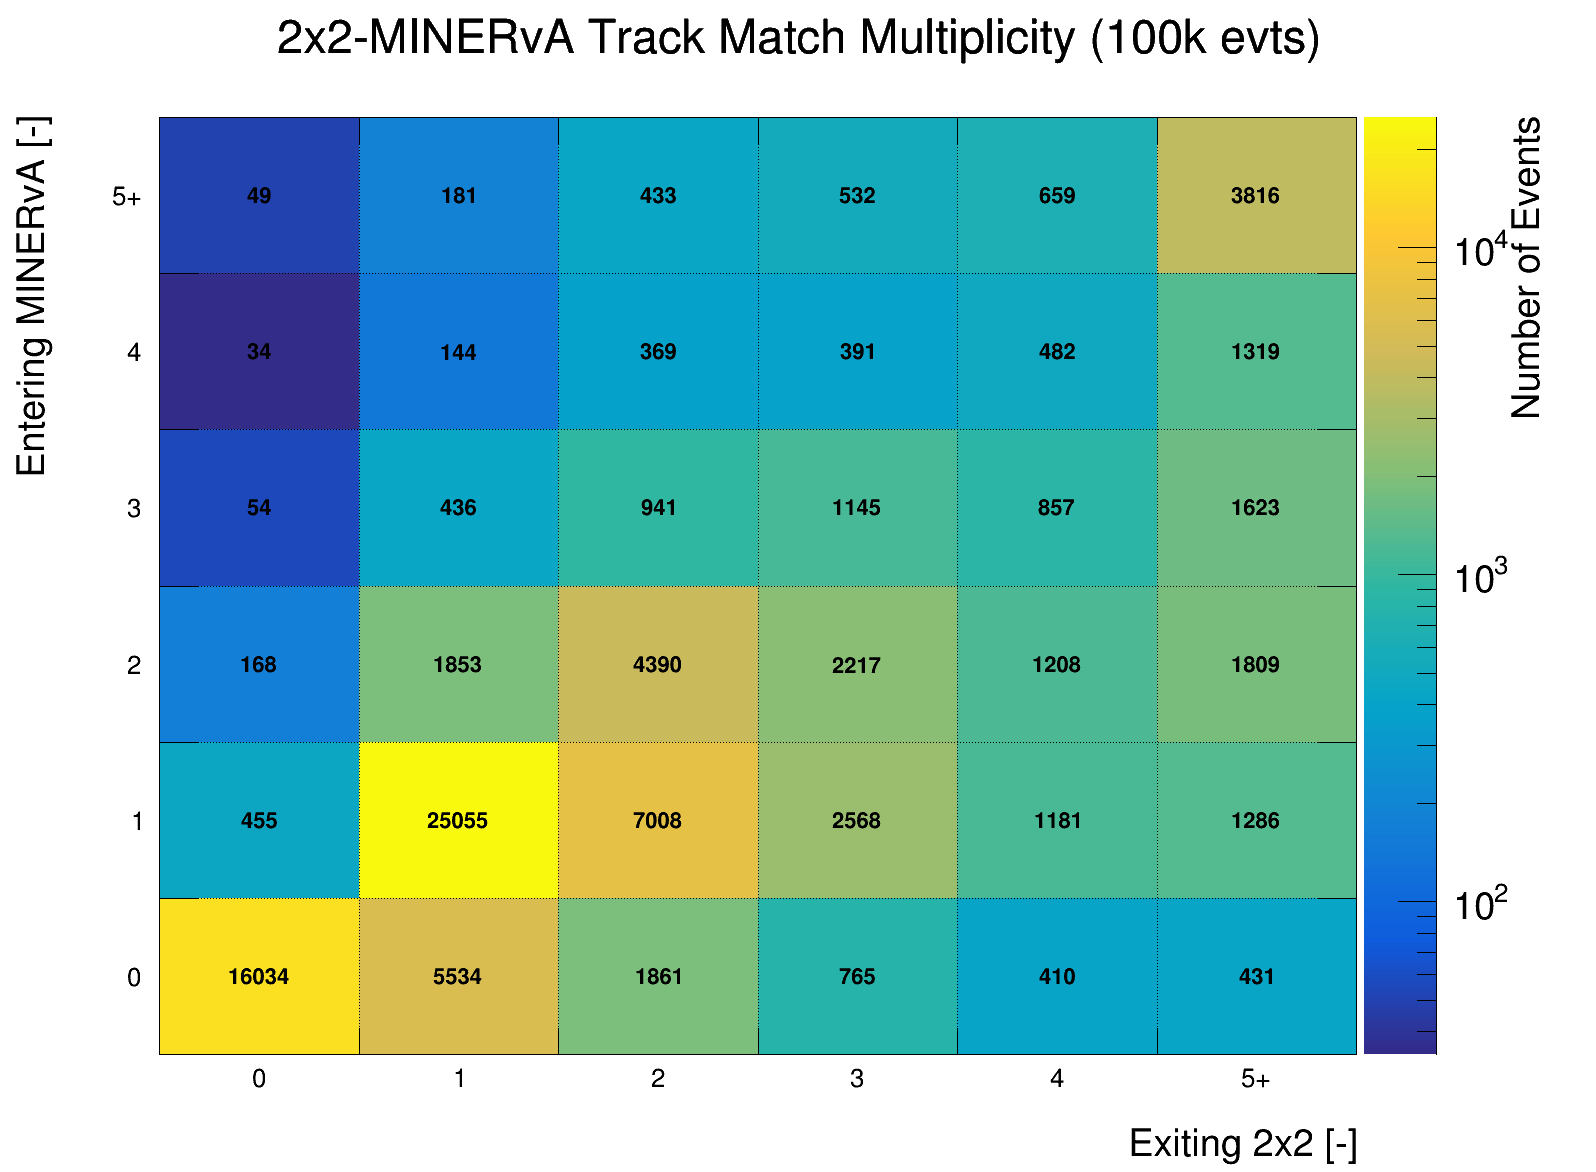
\includegraphics[width=0.6\textwidth]{plots/2x2_minerva_plots/track_mathch_topo.png}
  \caption{Simulated number of true tracks produced by simulated GENIE interactions in the ArgonCube 2x2 active volume, which exit the downstream face of the 2x2 module, relative to the number of tracks which enter the upstream face of the downstream ProtoDUNE-ND-Tracker, event by event.}
  \label{fig:track_multiplicity_topo}
\end{figure}
As can be seen from the event display shown in Figure~\ref{fig:2x2+MINERvA_event}, tracks which escape the ArgonCube 2x2 active volume may re-interact in the surrounding LAr bath before entering the ProtoDUNE-ND-Tracker, thus making the event more confusing, and difficult to assess reconstruction performance with. Figure~\ref{fig:track_multiplicity_topo} shows the multiplicity of tracks exiting the downstream face of the 2x2 active volume downstream, compared with the number of tracks entering the upstream face of the ProtoDUNE-ND-Tracker. The distribution is fairly diagonal, suggesting that although complicated event topologies exist, the events will not be too confused to use for these studies. Note also that this problem could be dramatically reduced by partially instrumenting the dead region between the two detectors.

\subsection{Acceptance studies}
\label{sec:minerva-acceptance}
The inclusion of ProtoDUNE-ND-Tracker in ProtoDUNE-ND will improve the acceptance of particles for various studies. Here, we show how the efficiency for contained events compares for the 2x2+Tracker setup described above, and for the 2x2-only case.

\begin{figure}[htb]
  \centering
  \subfloat[2x2-only]    {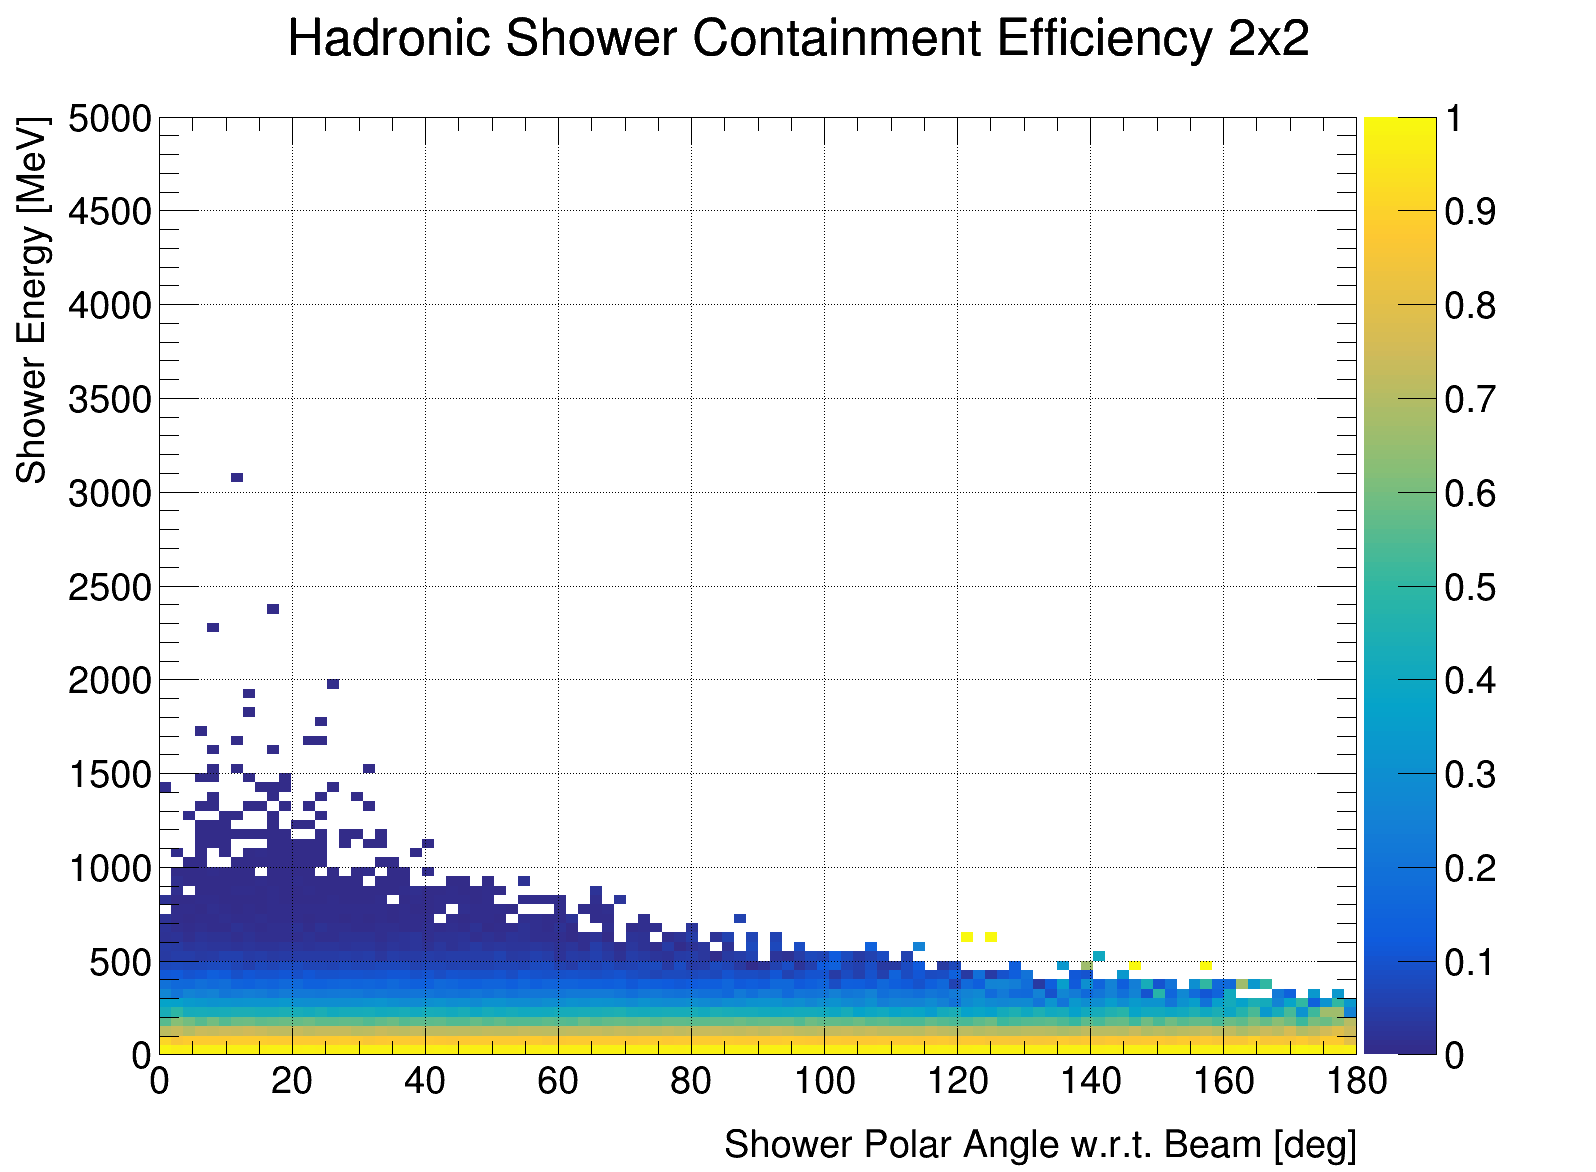
\includegraphics[width=0.45\textwidth]{plots/2x2_minerva_plots/H_cont_eff_2x2.png}}
  \subfloat[2x2+Tracker] {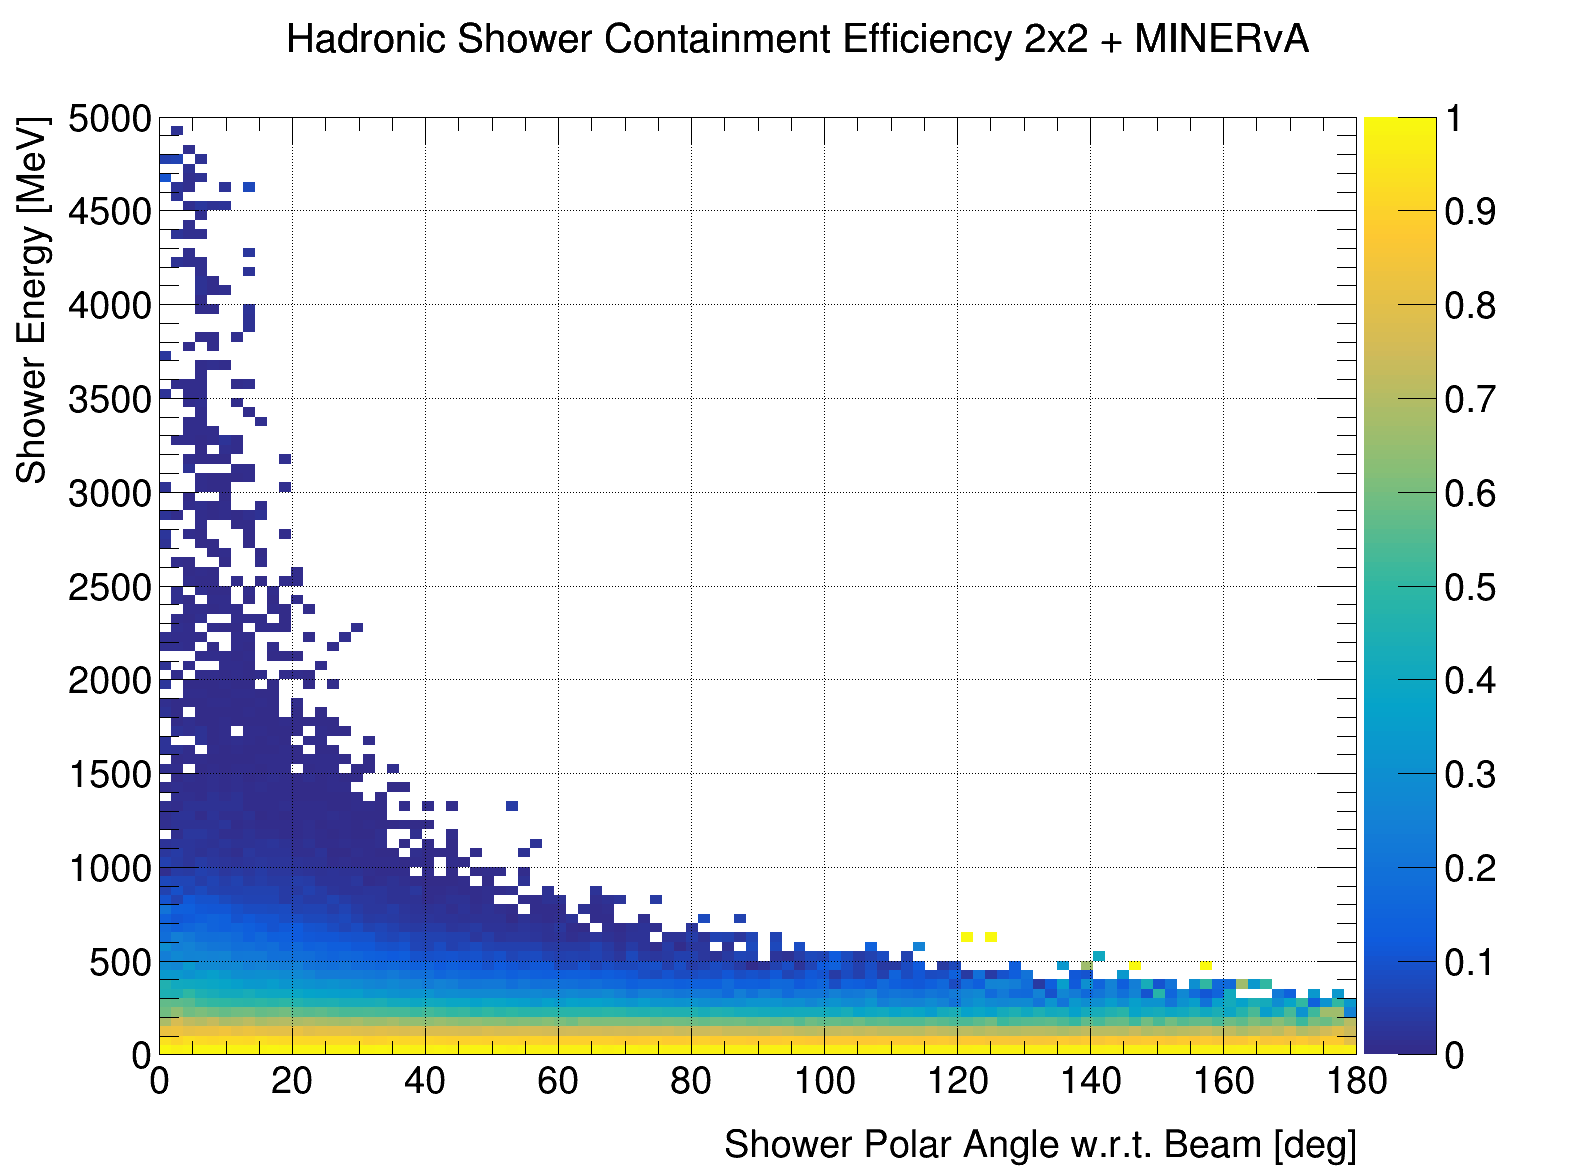
\includegraphics[width=0.45\textwidth]{plots/2x2_minerva_plots/H_cont_eff_2x2_MINERvA.png}}
  \caption{Efficiency for containing hadronic showers, in the ArgonCube 2x2-only, and ArgonCube 2x2+Tracker, as a function of hadronic shower energy and angle w.r.t the incoming neutrino direction. Containment is defined as $\geq$90\% of the energy being deposited in an active volume of a detector.}
  \label{fig:hadronic_containment}
\end{figure}
In Figure~\ref{fig:hadronic_containment}, the containment of hadron-induced showers is shown as a function of the true energy of the shower, and its angle w.r.t the incoming neutrino beam direction. Showers are defined as being contained when $\geq$90\% of the true energy of the shower is deposited inside the active 2x2 volume, or the ProtoDUNE-ND-Tracker if applicable. As expected, including the ProtoDUNE-ND-Tracker downstream of the 2x2 module increases the efficiency for angles $\theta \lesssim 30^{\circ}$, which dramatically increases the containment of high energy $E \gtrsim 0.5$ GeV hadronic showers, which tend to be forward-going.

\begin{figure}[htb]
  \centering
  \subfloat[2x2-only]    {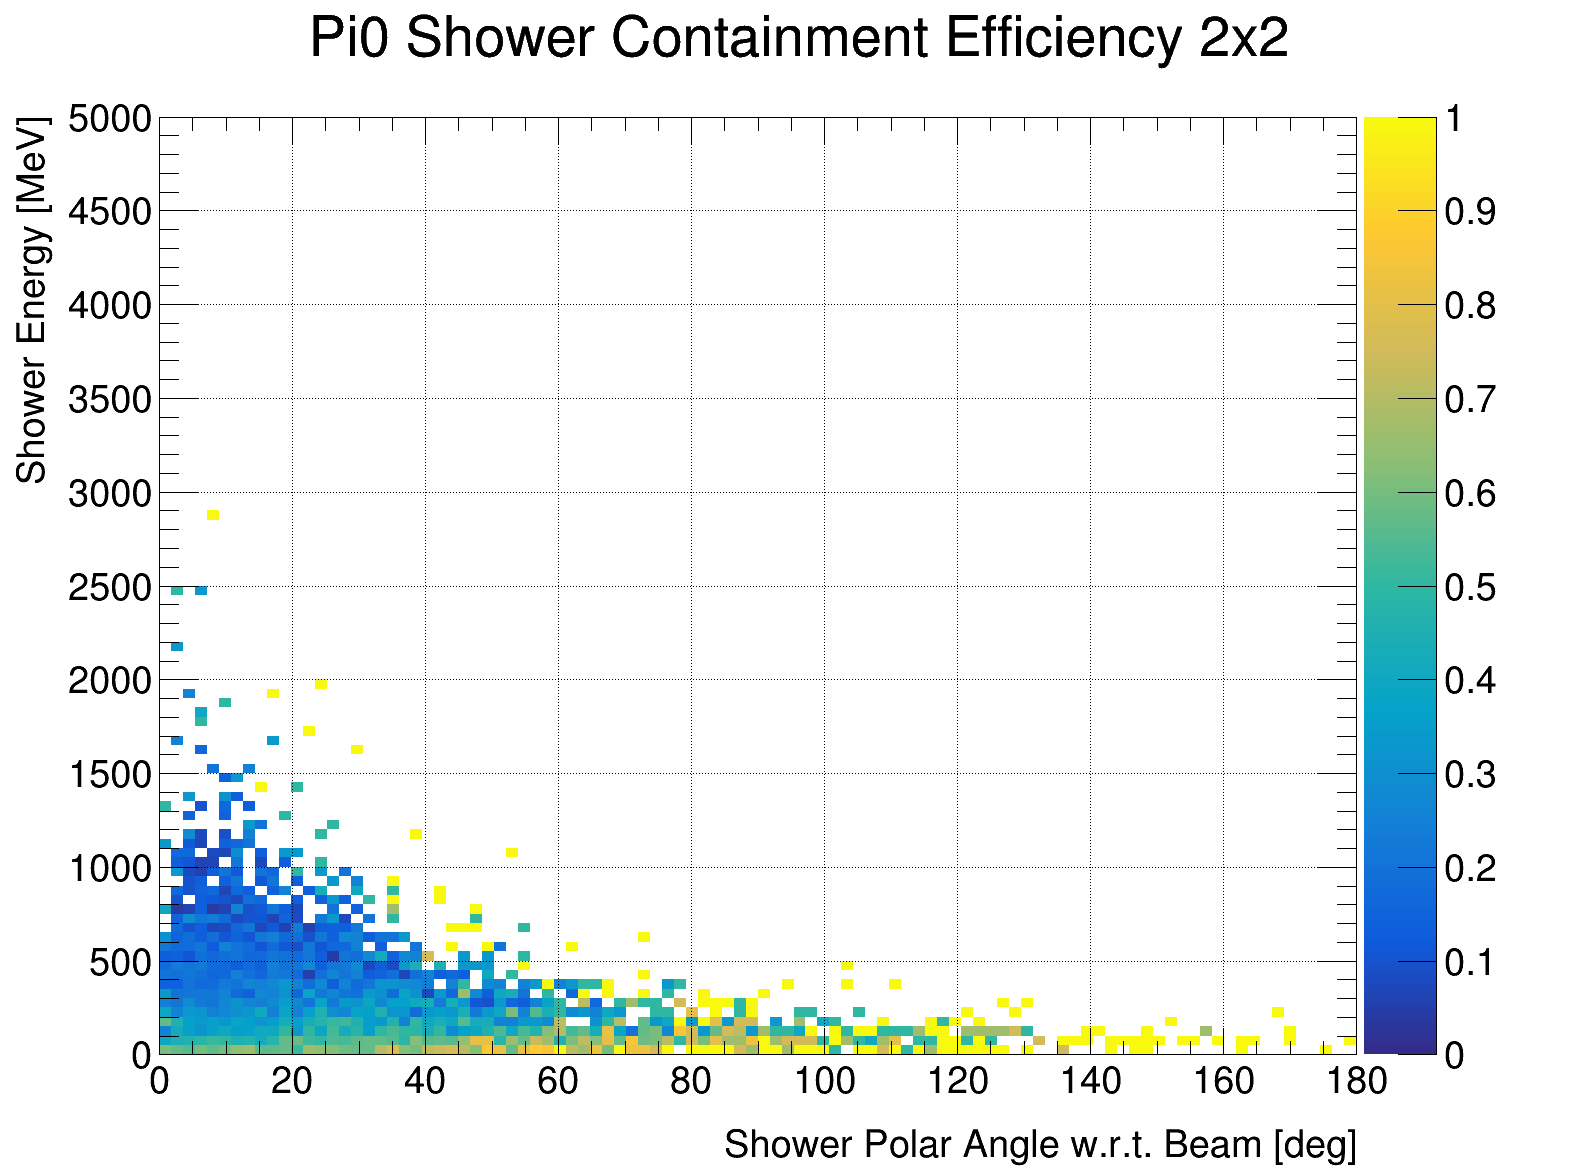
\includegraphics[width=0.45\textwidth]{plots/2x2_minerva_plots/Pi0_cont_eff_2x2.png}}
  \subfloat[2x2+Tracker] {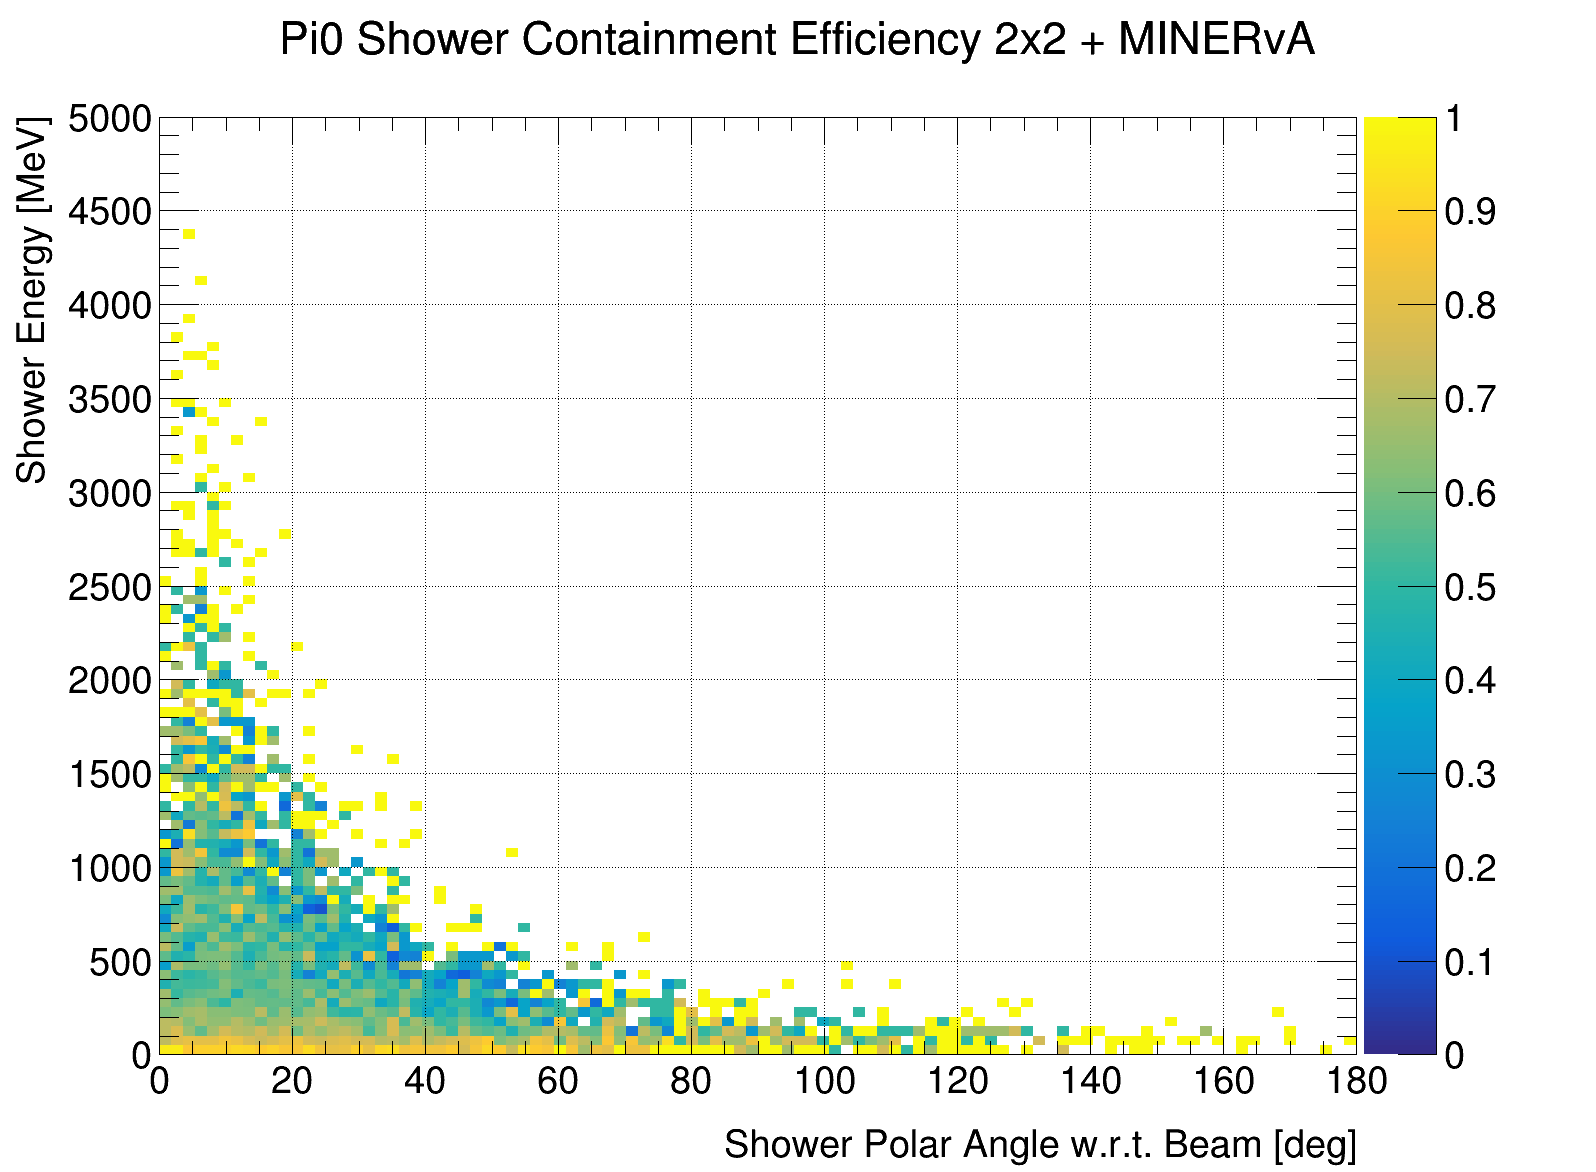
\includegraphics[width=0.45\textwidth]{plots/2x2_minerva_plots/Pi0_cont_eff_2x2_MINERvA.png}}
  \caption{Efficiency for containing both photon-induced showers from $\pi^{0}$ decays, in the 2x2-only, and 2x2+Tracker, as a function of the $\pi^{0}$ kinetic energy and angle w.r.t the incoming neutrino direction. Containment is defined as $\geq$90\% of the energy being deposited in an active volume of a detector.}
  \label{fig:pi0_containment}
\end{figure}
As discussed in Ref.~\cite{2x2@FNAL}, as the ArgonCube 2x2 module will not be placed in a test beam prior to installation in the NuMI beam at Fermilab, measurements in which the energy scale of the 2x2 can be calibration will be vital to assess the quality of energy reconstruction in the detector. The containment of both photons from a $\pi^{0}$ decay provides an appropriate in situ measurment of the energy reconstruction capabilities. In Figure~\ref{fig:pi0_containment}, the efficiency to contain 90\% of the energy from both photon-induced showers from a $\pi^{0}$ decay within the active volume of the 2x2, or the ProtoDUNE-ND-Tracker if relevant, is shown as a function of the $\pi^{0}$ kinetic energy and angle w.r.t the incoming neutrino beam. There is a significant increase in efficiency for all kinetic energies above a few hundred MeV, particularly for high energy ($E_{\pi^{0}} \gtrsim 1$ GeV) pions, which are produced in the forward direction. Although the dead space between the ArgonCube 2x2 active volume and the ProtoDUNE-ND-Tracker complicates this picture somewhat, it is clear that including the ProtoDUNE-ND-Tracker would give much greater statistics for this benchmark test of the ArgonCube detector performance.

\subsection{Neutron tagging studies}

\begin{figure}[htb]
  \centering
  \subfloat[2x2]    {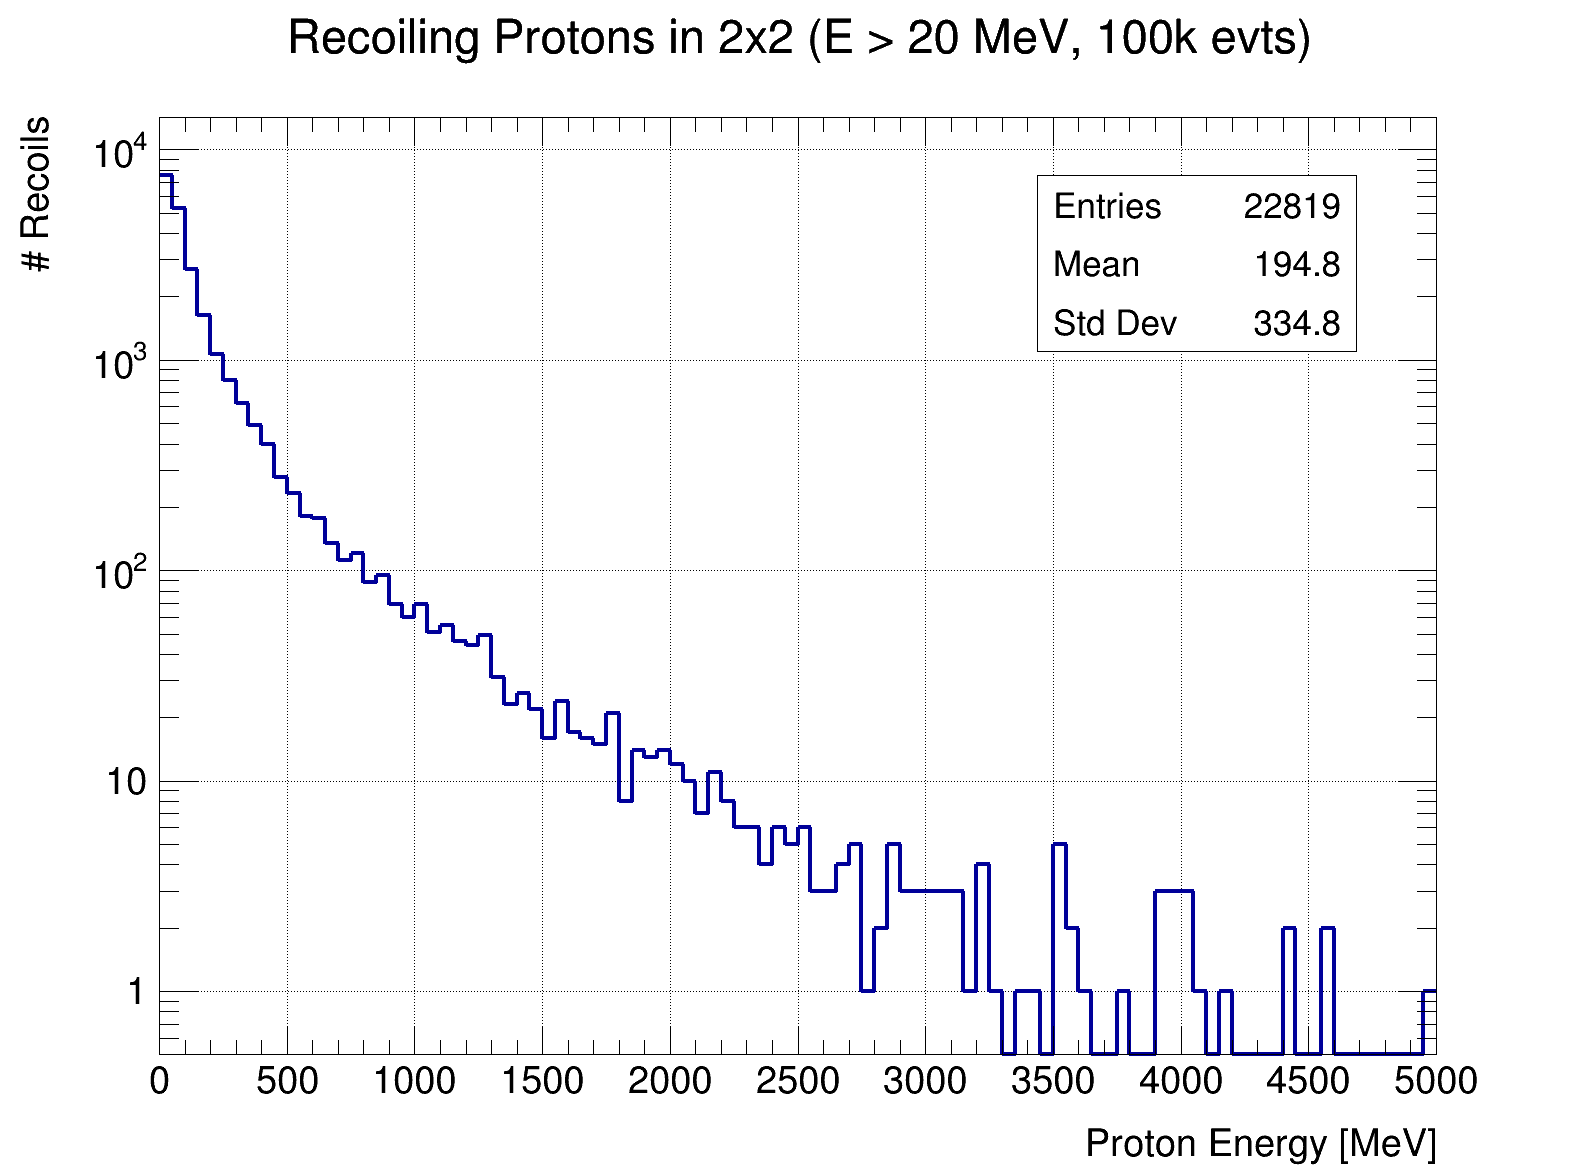
\includegraphics[width=0.45\textwidth]{plots/2x2_minerva_plots/recoils_vs_E_proton_2x2.png}}
  \subfloat[ProtoDUNE-ND-Tracker] {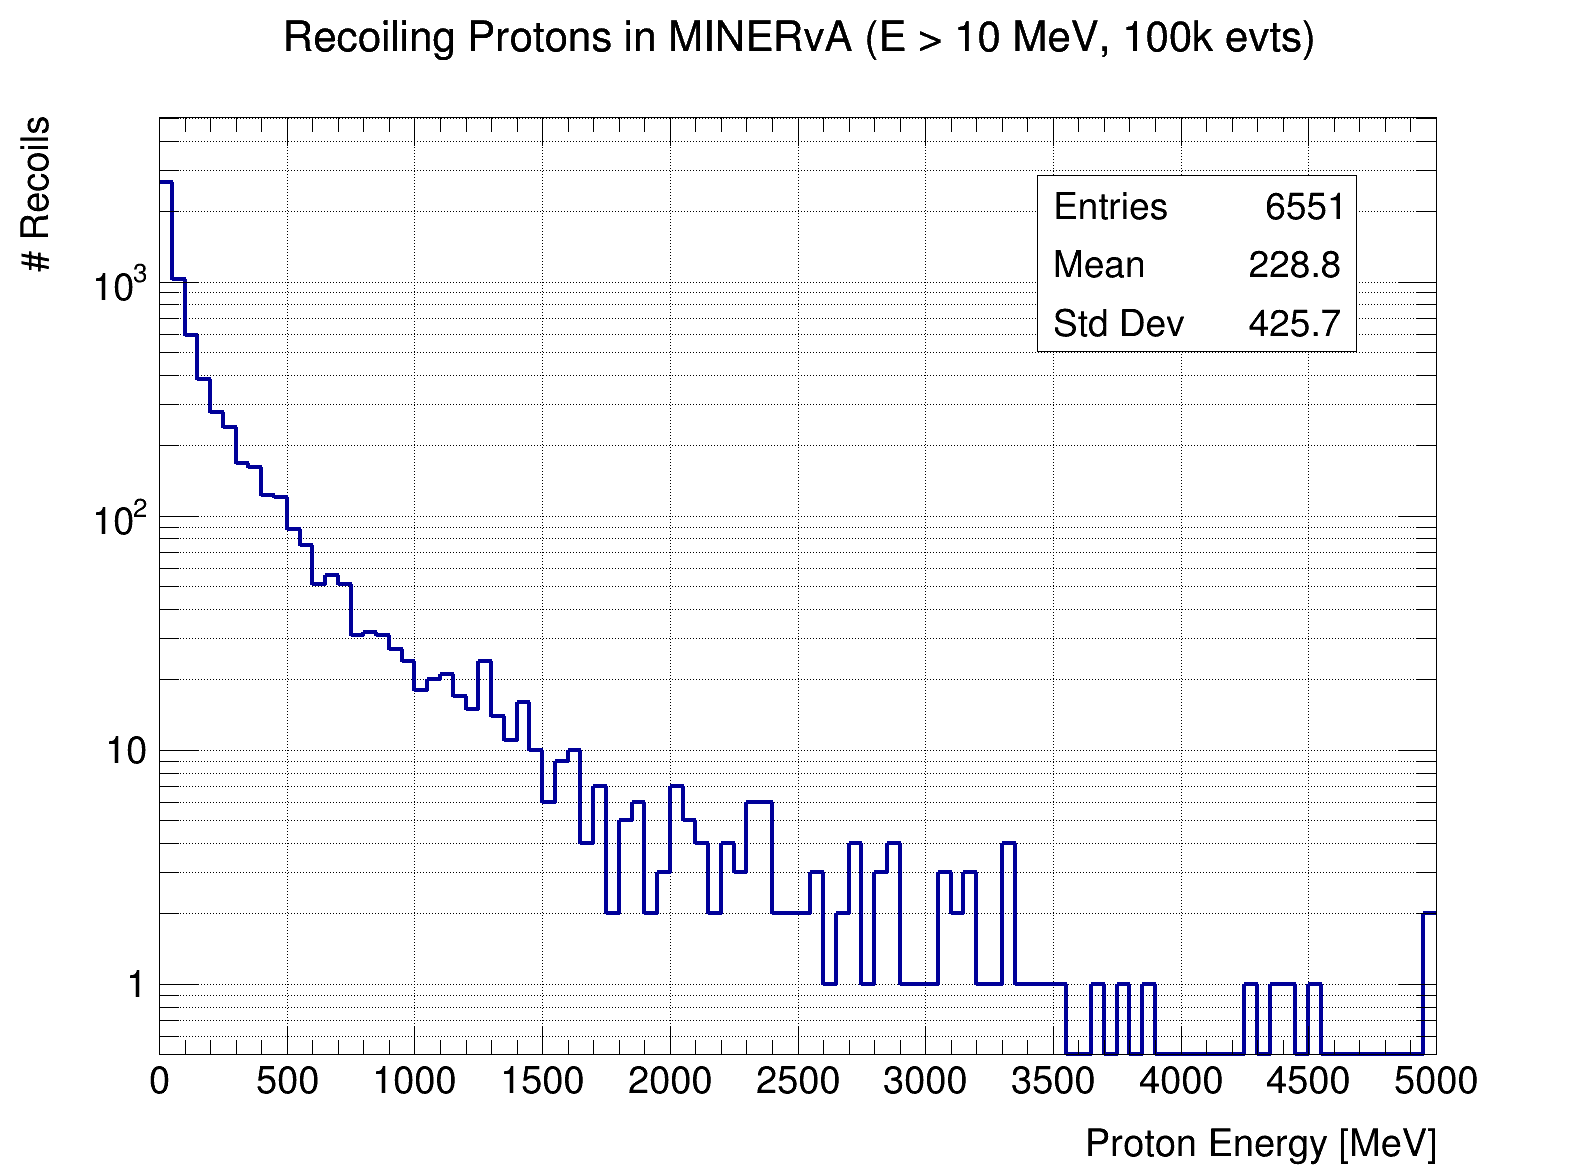
\includegraphics[width=0.45\textwidth]{plots/2x2_minerva_plots/recoils_vs_E_proton_MINERvA.png}}
  \caption{Number of neutron-induced proton recoils as a function of proton energy, which originate from an interaction vertex in the 2x2 active volume, seen in both the 2x2 ative volume, and the downstream ProtoDUNE-ND-Tracker.}
  \label{fig:neutron_tag_minerva}
\end{figure}

As discussed in Ref.~\cite{2x2@FNAL}, one key detector physics goal with ProtoDUNE-ND is to determine whether neutron-induced proton recoils can be identified in a LAr TPC, specifically in ArgonCube. The ability to identify and measure neutrons produced in neutrino interactions is of great interest to DUNE.  At the far detector, recoil protons can be identified and easily associated to the neutrino interaction as there will minimal event pile-up.  However, at the near detector, confusion due to multiple neutrino interactions in the same beam spill poses a unique challenge.  Because neutrons can travel $\mathcal{O}\left(1\right)\,\mathrm{m}$ in LAr without interacting, and proton recoils from fast neutrons typically deposit energy on a single pixel and thus contain no directionality, event association is not possible without matching the charge deposit to an ArCLight optical flash with fast timing resolution.
 
Additionally, it may be possible to measure the neutron energy from time of flight in the DUNE ND using the ECAL with very fast, sub-nanosecond timing resolution. This will require matching muon tracks from either the LAr or HPgTPCs to hits in the ECAL to reconstruct the neutrino interaction vertex time with high precision, and also identify and timestamp a subsequent neutron interaction in the scintillator tiles of the ECAL. This would give the DUNE ND unprecedented ability to make measurements of the neutron energy spectrum in neutrino-argon interactions. This technique has not been tested in a high rate environment. Because the neutrons may propagate for $\mathcal{O}\left(10\right)\,\mathrm{ns}$, even a very fast detector may suffer from confusion due to pile-up.

The existing MINERvA detector can detect neutron-induced proton recoils down to energies of a few MeV, and measure the 3D position of a recoil with a threshold of 20~MeV.  MINERvA has an established neutron reconstruction and a relatively well-understood detector response, which will be carried over into the ProtoDUNE-ND-Tracker.  As shown in Fig. 24, it will be possible to reconstruct neutrons originating in the LAr of the ArgonCube 2x2 Demonstrator by their interactions in the ProtoDUNE-ND-Tracker. The ability to match both muons and neutrons originating in LAr to a fast-timing scintillator detector would be a direct test of the feasibility of this technique in DUNE ND. This has profound impact on the design of the ECAL, which would need to be optimized for both EM and neutron reconstruction if this technique is demonstrated to be viable. 
 
 
\FloatBarrier
